% IEEE standard conference template; to be used with:
%   spconf.sty  - LaTeX style file, and
%   IEEEbib.bst - IEEE bibliography style file.
% --------------------------------------------------------------------------

\documentclass[letterpaper]{article}
\usepackage[utf8]{inputenc}
\usepackage[OT1]{fontenc}
\usepackage{spconf}
\usepackage[american]{babel}
\usepackage[babel=true]{microtype}
\usepackage{amsmath,amssymb,amsfonts,amsthm,mathrsfs}
\usepackage{graphicx}
\usepackage[nospace]{varioref}
\usepackage{caption}
\usepackage{array}
\usepackage{booktabs}
\usepackage{enumitem}
\usepackage[autostyle=true]{csquotes}
\usepackage{tikz}
\usepackage{minted}
\usepackage{algorithm}% http://ctan.org/pkg/algorithm
\usepackage[noend]{algpseudocode}% http://ctan.org/pkg/algorithmicx
\usepackage{listings}

% listings stuff
\setminted{fontsize=\footnotesize}
\setminted{autogobble}
\setminted{linenos}

% algpseudocode stuff
\MakeRobust{\Call} % allow nested calls
\makeatletter
\renewcommand{\ALG@beginalgorithmic}{\small} % set smaller font size for pseudocode
\makeatother

\graphicspath{{figures/}} %Setting the graphicspath

% Example definitions.
% --------------------
% nice symbols for real and complex numbers
\newcommand{\R}[0]{\mathbb{R}}
\newcommand{\C}[0]{\mathbb{C}}

% bold paragraph titles
\newcommand{\mypar}[1]{{\bf #1.}}

% Title.
% ------
\title{Optimizing the General Floyd-Warshall Algorithm}
%
% Single address.
% ---------------
\name{Florian Bütler, Manuel Hässig, Lasse Meinen, Roman Niggli}
\address{Department of Computer Science\\ ETH Zurich, Switzerland}

% For example:
% ------------
%\address{School\\
%		 Department\\
%		 Address}
%
% Two addresses (uncomment and modify for two-address case).
% ----------------------------------------------------------
%\twoauthors
%  {A. Author-one, B. Author-two\sthanks{Thanks to XYZ agency for funding.}}
%		 {School A-B\\
%		 Department A-B\\
%		 Address A-B}
%  {C. Author-three, D. Author-four\sthanks{The fourth author performed the work
%		 while at ...}}
%		 {School C-D\\
%		 Department C-D\\
%		 Address C-D}
%

\begin{document}
%\ninept
%
\maketitle
%

\begin{abstract}
The Floyd-Warshall algorithm is a widely used way of solving the all-pairs-shortest-path problem. Due to its popularity, much research has been done on ways to optimize the algorithm.
In addition, the Floyd-Warshall algorithm is proven effective at solving a wide range of other problems, by simply replacing its input type and basic operations.

In this work, we implement several known optimization techniques on the all-pairs-shortest-path Floyd-Warshall, and confirm their effectiveness. We also implement these techniques on two other instances of the Floyd-Warshall algorithm, namely transitive closure  and all-pairs-widest-path. We evaluate the optimizations on these two instances and confirm that they work on Floyd-Warshall instances beyond all-pairs-shortest-path.

Finally, we present an autotuner that empirically finds good parameters for several optimization strategies, and generates functional, optimized code for all three implementations.
\end{abstract}
\section{Introduction}\label{sec:intro}
The well-known Floyd-Warshall algorithm \cite{floyd62shortest} for computing the all-pairs shortest path problem
underlies a more general structure that solves several related problems. Some examples are the computation of the
transitive closure of a graph \cite{warshall62boolean, roy1959transitivite}, the computation of the widest path
\cite{pollack60widest}, Kleene's algorithm to transform a nondeterministic automaton to a regular expression
\cite{kleene1956representation} or the inversion of a matrix using the Gauss-Jordan method. Lehmann
\cite{lehmann77algebraic} relates these algorithms using the notion of computing the \emph{closure of a matrix}
with respect to a closed semi-ring.
The computation of the closure with the Floyd-Warshall method is a $k$-$i$-$j$ nested loop where the computation in
the innermost loop uses the operations of a particular closed semi-ring suitable to a given application.

\mypar{Motivation}
In the era without free speedup due to Moore's law where we have hit the memory, instruction level parallelism, and power walls, it is
as important as ever to write optimized programs to fully take advantage of the power of today's computers.
However, optimizing numerical code often leads to a large
unreadable tangled mess of unrolled and tiled loops, and single-static-assignment style code. Moreover, writing programs with very large
unrolling factors stops being just boring and becomes downright infeasible to do by hand.

The natural reaction to this is of course to automate the process of writing highly optimized code. Generating
optimized programs using autotuners, which generate a program specifically optimized for a given machine
configuration. However, algorithm specific autotuners need to be reimplemented for
each new algorithm, which often is a significant undertaking.

However, with sufficient structural similarity between algorithms (e.g. identical loop structure,
similar data representation, instruction latency and throughput) the same optimizations techniques should intuitively
lead to good results for all similar algorithms. For example, consider different algorithms with nested loops
where the inner loop performs different operations. An autotuner capable of unrolling loop in the
loop structure of this class of algorithm can optimize the unrolling factors for all such algorithms.

In this work we aim to exploit the structural similarity between the specializations of the general
Floyd-Warshall algorithm using different closed semi-rings to apply the same optimizations to a whole
class of algorithms. 

\mypar{Contribution}
In this work we optimize implementations of the shortest-path, transitive closure and widest path algorithm
by applying unrolling, cache tiling, and vectorization. Further, we present an autotuner which finds locally
optimal unrolling and tiling parameters for a given machine.

We aim to exploit the similarities between the algorithms given the common framework of a matrix closure by
writing an autotuner that is able to apply these optimizations to all three algorithms, i.e. all three closed
semi-rings. With this autotuner we demonstrate the potential to reuse a general enough autotuner on a class
of algorithms.

\mypar{Related Work}
The closed semi-rings Lehmann introduces in \cite{lehmann77algebraic} are a subcategory of Kleene-algebras.
Kozen provides a survey \cite{kozen1990kleene} about Kleene-algebras, their applications and how closed
semi-rings relate to them. For an approachable introduction to algorithms based on matrix closure consider
\cite{aho1974design, mehlhorn1984algo}. Further, Dolan \cite{dolan2013fun} implements a host of
algorithms based on the closure on closed semi-rings.

There have been several works to autotune single-core numerical computations, especially linear algebra
subprograms. In his PhD thesis, Nelson \cite{nelson2015dsl} provides a good summary of past efforts.
Related to the all-pairs shortest path problem, the Han, Franzetti, and Püschel \cite{han06generation}
created an autotuner for the Floyd-Warshall algorithm and applied unrolling and cache tiling,
notably removing the k-loop dependency based on techniques from \cite{venkataraman2000blocked, park2004cache}.


%While best known for solving the all-pairs-shortest-path problem, the Floyd-Warshall algorithm can be applied on a wide range of problems, as the algorithm essentially computes the transitive closure of a matrix over a closed semi-ring.
%Hence, by varying the underlying semi-ring, the algorithm can easily be adapted to suit the task at hand, making it one of the more widely used algorithms in computer science. % TODO: examples here
%
%Due to its ubiquity in modern computing, it is especially important to have access to efficient implementations. Depending on the use-case, these implementations have to process matrices of tremendous size. And especially in these cases, performing implementations have to be able to scale with large input sizes as well.
%
%In this work, we focus our work on three instances of the Floyd-Warshall algorithm, each arising from its own semi-ring:
%\begin{itemize}
%\item The shortest-path problem, corresponding to the semi-ring \(\langle\mathbb{R}^{\infty},\,\min,\,+\rangle\)
%\item The widest-path problem, corresponding to the semi-ring \(\langle\mathbb{R}^{\infty},\,\max,\,\min\rangle\)
%\item The transitive-closure, corresponding to the semi-ring \(\langle\{0, 1\},\,\lor,\, \land\rangle\)
%\end{itemize}
%On each we first apply a few basic optimizations, namely loop unrolling and vectorization. We then implement more advanced optimizations with tiling. Finally, we present an autotuner, capable of searching for locally optimal meta parameters, and generating functional C code with these parameters.

%\mypar{Related Work}
%Lehman \cite{lehmann77algebraic} shows that the Floyd-Warshall algorithm computes the transitive closure of a matrix over a closed semi-ring, and relates it to the Gauss-Jordan method for inverting a matrix.
%Sung-Chul Han et al. \cite{han06generation} show how \emph{tiling} allows for several advanced optimizations of the Floyd-Warshall shortest path algorithm.
%They also present an automatic program generator, capable of significantly oupterforming hand-tuned implementations.
%
%%%%%%

%Do not start the introduction with the abstract or a slightly modified
%version. What follows is a possible structure of the introduction.
%This structure can be modified, but the content should be the same. The introduction should definitely end on the first page.
%
%\mypar{Motivation} The first task is to motivate what you do.  You can
%start general and zoom in one the specific problem you consider.  In
%the process you should have explained to the reader: what you are doing,
%why you are doing, why it is important (order is usually reversed).
%
%For example, if my result is the fastest DFT implementation ever, one
%could roughly go as follows. First explain why the DFT is important
%(used everywhere with a few examples) and why performance matters (large datasets,
%realtime). Then explain that fast implementations are very hard and
%expensive to get (memory hierarchy, vector, parallel).
%
%\mypar{Contribution}
%Now you state what you do in this paper. In our example:
%presenting a DFT implementation that is
%faster for some sizes than all the other ones.
%
%\mypar{Related work} Next, you have to give a brief overview of
%related work. For a paper like this, anywhere between 2 and 8
%references. Briefly explain what they do. In the end contrast to what
%you do to make now precisely clear what your contribution is.

\section{Background on Warshall-Floyd-Kleene's Algorithm}\label{sec:background}

In this section, we give short definition of closed semi-rings, define the structure of the
generalized standard Floyd-Warshall (FW) algorithm, present the two alternative versions we use
and perform a simple cost analysis.

\mypar{Closed semi-rings}
A closed semi-ring is an algebra $\langle R,+,\cdot,*,0,1\rangle$, where $R$ is a set,
$+: R \times R \rightarrow R$ and $\cdot: R \times R \rightarrow R$ are binary operations
called addition and multiplication, resp., $*: R \rightarrow R$ is a unary operation
called closure, and $0 \in R$, $1 \in R$ are constants. The algebra must fulfil the
following axioms:
\begin{itemize}
    \item $\langle R, + \rangle$ is a commutative monoid with identity element 0:
            \begin{itemize}[noitemsep,topsep=0pt]
                \item $a + (b + c) = (a + b) + c$
                \item $a + b = b + a$
                \item $a + 0 = a$
            \end{itemize}
    \item $\langle R, \cdot \rangle$ is a monoid with identity element 1:
             \begin{itemize}[noitemsep,topsep=0pt]
                 \item $(a \cdot b) \cdot c = a \cdot (b \cdot c)$
                 \item $1 \cdot a = a = a \cdot 1$
             \end{itemize}
    \item Multiplication distributes over addition:
            \begin{itemize}[noitemsep,topsep=0pt]
                \item $a \cdot (b + c) = a \cdot b + a \cdot c = (b + c) \cdot a = b \cdot a + c \cdot a$
            \end{itemize}
    \item Closure satisfies the following equation:\\
        $a^* = 1 + a \cdot a^* = 1 + a^* \cdot a$
\end{itemize}
Lehman \cite{lehmann77algebraic} shows that the
Floyd-Warshall algorithm computes the closure of a matrix $A \in R^{N \times N}$
for any simple closed semi-ring over $R$. 

We introduce specific examples in the next section. For simplicity, we omit $*$, $0$
and $1$ from the algebra definitions, as all three can easily be deduced from
$\langle R, +, \cdot \rangle$.

\mypar{Generalized FW algorithm}
The generalized standard Floyd-Warshall algorithm can be seen in Alg. \ref{alg:fw}.
It consists of three nested loops, where the outermost loop updates each entry in
the $N \times N$ matrix C $N$ times, and \textit{cannot} be reordered with the two
inner loops. 

For a particular semi-ring \(\langle R,\,+,\,\cdot\rangle\), we create an instance
of the algorithm by setting \texttt{ADD} to be the additive operation $+$,
\texttt{MUL} to be the multiplicative operation $\cdot$, and \texttt{C} to be such
that $C \in R^{N \times N}$. For example, the generalized FW algorithm instantiated
with the semi-ring \(\langle\R^{\infty},\min,\,+\rangle\), where
\texttt{C} is the \textit{cost matrix} of the underlying graph, solves the all-pairs
shortest path (APSP) problem.

A comparison of the two algorithms reveals that the structure of the FW algorithm is
very similar to that of Matrix-Matrix Multiplication (MMM). Due to cache locality,
the loop order $k-i-j$ would to be changed to $i-j-k$, in order to achieve peak performance
as is the case for MMM. However, in the case of FW, the iterations of the outer loop
are not independent, that is, such a reordering without any other transformations
would result in an incorrect version of the algorithm.

\begin{algorithm}
  \caption{Structure of the generalized Floyd-Warshall algorithm.}\label{alg:fw}
  \begin{algorithmic}[1]
    \Function{floydWarshall}{$C,N$}
      \For{$k \gets 1$ to $N$}
      \EndFor
      \For{$i \gets 1$ to $N$}
      \EndFor
      \For{$j \gets 1$ to $N$}
        \State $C[i][j] \gets$ \Call{ADD}{$C[i][j]$, \Call{MUL}{$C[i][k]$, $C[k][j]$}}
      \EndFor
    \EndFunction
  \end{algorithmic}
\end{algorithm}

\mypar{Iterative FW algorithm: FWI}
Han, Franchetti and Püschel \cite{han06generation} introduced a tiled and unrolled
version of the FW algorithm for the APSP problem. For simplicity, we repeat its definition
here for the generalized version, which can be seen in Alg. \ref{alg:fwi}. The generalized
FWI algorithm introduces two variations on the standard FW algorithm. First, to facilitate
tiling in later optimizations, we now iterate over matrices \texttt{A}, \texttt{B} and
\texttt{C}. The matrix \texttt{A} contains the distances from \texttt{i} to \texttt{k},
\texttt{B} those from \texttt{k} to \texttt{j}, and \texttt{C} those from \texttt{i} to
\texttt{j}. Second, the two innermost loops are unrolled by factors $U_i$ and $U_j$, respectively.

We further introduce a special version of FWI, algorithm \ref{alg:fwiabc} FWIabc, which assumes that
matrices \texttt{A}, \texttt{B} and \texttt{C} \emph{do not} alias. Under this assumption,
we can reorder the three loops. Thus, we can now additionally unroll the \texttt{k}-loop.

For simplicity, we assume the unrolling factors $U_i$, $U_j$, $U_i^\prime$, $U_j^\prime$,
$U_k^\prime$ divide the matrix size $N$.

\begin{algorithm}
  \caption{FWI parameterized by unrolling parameters $U_i$, $U_j$ and semi-ring parameters \texttt{ADD}, \texttt{MUL}.}\label{alg:fwi}
  \begin{algorithmic}[1]
    \Function{FWI}{$A,B,C,N$}
      \For{$k \gets 1$ to $N$}
      \EndFor
      \For{$i \gets 1$ to $N$}
      \EndFor
      \For{$j \gets 1$ to $N$}
        \Statex\Comment{Loops below are completely unrolled}
        \For{$i^\prime \gets i$ to $i + U_i - 1$}
        \EndFor
        \For{$j^\prime \gets j$ to $j + U_j - 1$}
          \State $C[i^\prime][j^\prime] \gets$ \Call{ADD}{$C[i^\prime][j^\prime]$, \Call{MUL}{$A[i^\prime][k]$, $B[k][j^\prime]$}}
        \EndFor
      \EndFor
    \EndFunction
  \end{algorithmic}
\end{algorithm}

\begin{algorithm}
  \caption{FWIabc parametrized by unrolling parameters $U_i^\prime$, $U_j^\prime$, $U_k^\prime$ and semi-ring parameters \texttt{ADD}, \texttt{MUL}.}\label{alg:fwiabc}
  \begin{algorithmic}[1]
    \Function{FWIabc}{$A,B,C,N$}\Comment{$A,B,C$ do not alias}
      \For{$i \gets 1$ to $N$}
      \EndFor
      \For{$j \gets 1$ to $N$}
      \EndFor
      \For{$k \gets 1$ to $N$}
        \Statex\Comment{Loops below are completely unrolled}
        \For{$i^\prime \gets i$ to $i + U_i^\prime - 1$}
        \EndFor
        \For{$j^\prime \gets j$ to $j + U_j^\prime - 1$}
        \EndFor
        \For{$k^\prime \gets j$ to $k + U_k^\prime - 1$}
          \State $C[i^\prime][j^\prime] \gets$ \Call{OP1}{$C[i^\prime][j^\prime]$, \Call{OP2}{$A[i^\prime][k^\prime]$, $B[k^\prime][j^\prime]$}}
        \EndFor
      \EndFor
    \EndFunction
  \end{algorithmic}
\end{algorithm}

\mypar{Tiled FW algorithm: FWT}
Building on the previously introduced algorithms, Han, Franchetti and Püschel
\cite{han06generation} introduced a singly cache-tiled version of the FW algorithm. We
again state its definition here for the generalized version. The algorithm \ref{alg:fwt} FWT
iterates over tiles of size $L1 \times L1$,
proceeding in four phases. In the first phase, the diagonal tile $C_{kk}$ is updated.
In the second and third phases, the tiles in the column and row of $C_{kk}$ are updated.
In the fourth phase, all remaining tiles are updated. The three tiles under
consideration are guaranteed to be independent in the fourth phase and we can therefore
use the \texttt{FWIabc} subroutine. Note that the fourth phase encompasses the bulk of
the computation. Therefore, this separation of the algorithm into four phases allows us to run
the majority of the computation without the aforementioned outer-loop dependency.

For simplicity, we assume the tile size $L1$ divides the matrix size $N$.

\begin{algorithm}
  \caption{FWT parameterized by tile size $L1$, and the parameters for \texttt{FWI} and \texttt{FWIabc}}\label{alg:fwt}
  \begin{algorithmic}[1]
    \Function{FWT}{$A,B,C,N,L1$}
      \State // $A_{ij}$: $L1 \times L1$ submatrix $(i,j)$ of $A$
      \State $M\gets N/L1$
      \For{$k \gets 1$ to $M$}
        \State \Call{FWI}{$A_{kk}, B_{kk}, C_{kk}, L1$}
        \Comment{Phase 1}
        \For{$j \gets 1$ to $M$, $j \neq k$}
          \State \Call{FWI}{$A_{kk}, B_{kj}, C_{kj}, L1$}
          \Comment{Phase 2}
        \EndFor
        \For{$i \gets 1$ to $M$, $i \neq k$}
          \State \Call{FWI}{$A_{ik}, B_{kk}, C_{ik}, L1$}
          \Comment{Phase 3}
        \EndFor
        \For{$i \gets 1$ to $M$, $i \neq k$}
        \For{$j \gets 1$ to $M$, $j \neq k$}
          \State \Call{FWIabc}{$A_{ik}, B_{kj}, C_{ij}, L1$}
          \Comment{Phase 4}
        \EndFor
        \EndFor
      \EndFor
    \EndFunction
  \end{algorithmic}
\end{algorithm}

\mypar{Cost Analysis}
We define the cost of the FW algorithm to be the total number of operations on the
semi-ring, that is, the number of \texttt{ADD} and \texttt{MUL} operations.
%%%%% we changed that
%Please
%note that for the (bit-packed) transitive closure implementation, we counted one
%operation per byte (as opposed to per element) to simplify calculations regarding
%theoretically achievable peak performance.
Note that if the additive and
multiplicative operations are not equally expensive in terms of the number of CPU
cycles on a particular system, this cost measure will not accurately represent the
performance of an implementation. In our case, however, this does not pose a problem,
as the two operations are equal in cost for all three FW instances under consideration.

The general FW algorithm consists of three nested loops with two operations in the
innermost loop and therefore we have $2N^3$ operations according to our cost function.
Thus, it is trivial to see that the asymptotic complexity of the FW
algorithm is $\mathcal{O}(N^3)$. As this report does not deal with instances of the FW
algorithm for sparse matrices, the upper asymptotic bound simplifies to a tight one.

\section{Method}\label{sec:yourmethod}
In this section, start with an overview of the FW instances we examine, and the infrastructure we work with. Then, we briefly describe our process of writing baseline implementations, and then implementing various optimizations.

This work is focused on three particular semi-rings, each giving rise to its own instance of the Floyd-Warshall algorithm, targeted at solving its own problem.
\begin{itemize}
\item The semi-ring \(\langle \mathbb{R}^{\infty},\min,+\rangle\) corresponds to the all-pairs \emph{shortest-path problem} (APSP). It computes the length of the shortest path between every pair of vertices in a graph.
\item The semi-ring \(\langle \mathbb{R}^{\infty},\max,\min\rangle\) corresponds to the all-pairs \emph{widest-path problem} (MM). It maximizes the smallest weight, a path between every pair of vertices has.
\item The semi-ring \(\langle \{0, 1\},\lor,\land\rangle\) corresponds to the \emph{transitive closure} (TC). It checks for every pair of vertices, if one is reachable from the other.
\end{itemize}

For each of these three semi-rings, we start by writing simple reference implementations in \emph{Python} and \emph{Go}. These are not used for benchmarking purposes, but to ensure our later implementations are correct and produce the same results.

Next, we write and benchmark a naive baseline implementation for each semi-ring. Due to the algorithm's simplicity, many of the more standard optimization techniques like strength reduction or function inlining are not possible. For this reason, we optimize FW by implementing the previously introduced \texttt{FWI} and \texttt{FWT} algorithms for the three listed FW instances. Additionally, we implement vectorized versions of the resulting 6 implementations.

Lastly, we implement and evaluate an autotuner, which finds optimal parameters and generates code for \texttt{FWI}, \texttt{FWT}, and the corresponding vectorized versions.

\mypar{Setup}
Figure \ref{img:setup} illustrates our project setup. We generate input graphs with \emph{Python} and the \emph{networkx} library. Using our reference implementations, we compute correct outputs for each testcase.
To ensure our optimized implementations are correct, we run them against the same testcases and compare the results with the reference results.
Finally, we have a separate set of larger inputs, against which we benchmark the validated, optimized implementations.

Since boolean values require much less memory space than floating-point numbers, benchmarking the TC implementations requires much larger inputs than APSP and MM, which both operate on double-precision floating-point numbers.
Hence, storing input graphs for transitive closure the same way as for the other two problems would have been comically impractical - the larger graphs would have required several GB of space each.
To circumvent this issue, transitive closure implementations do not read any input when benchmarking for large input sizes. Instead, they simply allocate sufficient space to store the matrix to operate on, but do not overwrite it. This essentially provides random input data, which is perfect for our benchmarking purposes since the algorithm runtime is not dependent on the input values.

Please note that the reason this trick is possible for transitive closure, but not for the other two problems, is that computing the transitive closure on boolean values has no additional requirements on the underlying graph.
In comparison, APSP requires that the underlying graph does not have any \emph{negative cycles.} Of course, this makes sense: If a negative cycle exists in a graph, any connection can be routed through that cycle infinitely often, producing a shortest distance of \(-\infty\).

But beyond that, floating-point numbers also have a range of possible ways to represent values beyond numbers in \(\mathbb{R}^{\infty}\). To make sure, the APSP and MM implementations are always benchmarked on well-defined and suitable graphs, they are always run against previously generated matrices.
% And the way these values affect operations like addition, maximum or minimum is not always defined clearly. To prevent such situations from affecting the measurements, the shortest- and widest-path implementations are always run against well-defined and valid matrices.

To make all builds reproducible, implementations are compiled in docker. This ensures that compiler versions are consistent over all tested implementations.
% Depending on the implementation, they are also compiled with specific flags. For instance, implementations that do not use vector instructions are also compiled with flags that disallow the compiler from vectorizing the algorithm on its own.

\begin{figure}[h]
    \centering
    \includegraphics[width=0.4\textwidth]{img/setup.png}
    \caption{The Building, Testing and Benchmarking System}
    \label{img:setup}
\end{figure}

\mypar{Naive Implementation}
For APSP and MM, the naive implementation is as simple as possible, looking almost exactly like \ref{alg:fw}.
However, the naive implementation for TC already includes one optimization. The smallest datatype which C allows one to operate on is \texttt{char}. It has a size of 1 byte, or 8 bits.
But each of these bits is already enough to store a boolean value. The naive TC therefore already performs \emph{bit-packing}. That is a process wherein each byte accounts for 8 boolean values instead of just one.
This not only vastly reduces the space required to store and operate on matrices, but it also allows us to perform 8 logical operations at once, since taking the conjunction between two bytes actually performs eight bitwise conjunctions.

This is very similar to the later optimization of vectorization, as it essentially operates of vectors of 8 booleans each.

\mypar{Loop Unrolling}
Perhaps the most simple optimization performed in this project is \emph{loop unrolling}. Starting with the naive implementation, the two inner loops can be arbitrarily unrolled. But as mentioned earlier, the outermost loop cannot be unrolled, as it would violate dependencies.

In an additional, non-trivial optimization, the load of \texttt{C[i, k]} is moved out of the innermost loop. Furthermore, this value is not reloaded for the entire run of this loop.
At first, this optimization appears to be faulty, as the innermost loop can change \texttt{C[i, k]} if \texttt{j} is equal to \texttt{k}. However, in that case the update for APSP has the form of \texttt{C[i, k] = MIN(C[i, k], C[i, k] + C[k, k])}.
Since the algorithm requires the input graph not to have any negative circles, \texttt{C[k, k]} cannot be negative. Hence, \texttt{C[i, k] + C[k, k]} will never be smaller than just \texttt{C[i, k]}, meaning the update in question will never actually modify the value of \texttt{C[i, k]}.

For MM and TC, this optimization does not even require the input to fulfil any non-trivial problems. For MM, the update has the form \texttt{C[i, k] = MAX(C[i, k], MIN(C[i, k], C[k, k]))}, and for the TC it is \texttt{C[i, k] = C[i, k] | (C[i, k] \& C[k, k])}. In both cases, it is easy to see that the value of \texttt{C[i, k]} is left unchanged.

For easier understanding, a concrete example of unrolled code can be found in the appendix \ref{app:code}.

%At first, this implementation appears to be faulty: The value \texttt{cik = C[i, k]} is only read once for an entire run of the innermost loop. Yet, if the loop variable \texttt{j} is equal to \texttt{k}, the location \texttt{C[i, k]} can be overwritten. In such an event, it appears that \texttt{cik} would have to be read again, as its value might have changed. However, a closer examination of the problem at hand shows why this is not possible.
%The value that \texttt{C[i, k]} could be overwritten with, is computed as follows: \texttt{C[i, k] = MIN(C[i, k], C[i, k] + C[k, k])} (\emph{since we assume \texttt{k} and \texttt{j} are equal}). The only case in which this expression evaluates to something different from \texttt{C[i, k]} is if \texttt{C[k, k]} is negative. But since we explicitly require our graphs not to contain negative cycles, that is impossible.

\mypar{SIMD Vectorization}
\label{method:simd}
While certainly sounding more interesting, the introduction of SIMD (single instruction, multiple data) vector instructions is similar to just unrolling the innermost loop, but without all the additional load, compute and store statements. The unrolling factor depends on the data type the algorithm works with, as well as the hardware the program is to be run on.
For this project, we work with the \texttt{AVX} and \texttt{AVX2} vector instruction set, meaning the vector instructions work with vectors of 256 bits.
For the APSP and MM implementations, one such vector holds four doubles, meaning the innermost loops are essentially unrolled by a factor of four.
Regarding the TC, one such vector can hold 32 chars. This means that when compared to the naive implementation, the vectorized version unrolls the innermost loop by a factor of 32.

\mypar{Tiling}
This optimization is explained more thoroughly in section \ref{sec:background} and Alg. \ref{alg:fwt}. But in brief, the idea is to cut the matrix in tiles, and iterate over them. This not only allows for a faster loop ordering on some tiles, but if the tiles are of a suitable size, they also fit into the cache.
As a result, the processor has to spend significantly less time waiting for data, allowing it to more efficiently utilize its resources.

In addition to tiling, these implementations also have loop unrolling. In fact, using them with the tile size set to the entire input matrix is identical to using the unrolled version.

The tiled implementations are all parameterized by the tile size, which is set as high as possible such that three tiles fit into the machine's L2 cache.
To make the implementations more simple, we require the tile size divide the dimension of the input matrix, or the number of vertices in the input graph.
Furthermore, the tile size also has to be a multiple of the \emph{unrolling factor} of the functions operating on the tiles.

\mypar{Vectorized Tiling}
After the combination of tiling and unrolling, the obvious next step is to add vectorization too. As mentioned, vectorization is very similar to loop unrolling. The constraints on the tile size are therefore left unchanged for both the APSP and MM implementations.
However, in the case of TC, vectorization means that the unrolling factor becomes 256.
Coupled with the two constraints of dividing the input size and fitting into the cache, the vectorized tiled TC implementation is often forced to use significantly smaller tile sizes than would be optimal, leading to notable performance hits.
For a more stable implementation, the input matrix could be extended with zeros to allow for an optimal tile size. However, such an optimization is not part of this work.

\mypar{Autotuner}
In spite of the aforementioned constraints, there still is a vast number of possible parameters with which to implement a particular optimization, or a combination thereof.
Testing them all in order to find the best ones is therefore highly unpractical.
In addition, parameters that are optimal for one input size may not be the best for another size.
In order to find good parameters without tedious manual testing, we implement an autotuner, capable of testing parameters and searching good ones on its own.
While this autotuner is still unable perform an exhaustive search over all possible parameters, it can find locally optimal parameters and produce according code.

Figure \ref{img:autotuner} shows the process by which the autotuner formulates its guesses on suitable parameters, and then tries to refine them. It starts off by trying all possible parameters for an input size small enough to do so in reasonable time ($N=64$ in our case).
On the larger input size, the autotuner employs a hill-climbing algorithm to search for locally optimal parameters using the optimal parameter the algorithm found for a small input as an initial guess.
This algorithm again follows the illustrated process, where each round begins with the computation of parameter sets to try next. These parameter sets are generated by changing only one parameter of the current set, while leaving the rest unchanged. The new value for the changed parameter is always a neighbor of the current value, meaning either the next larger or next smaller value while respecting existing constraints.
In each round, the autotuner evaluates the performance on each of the generated parameter sets. If one of them surpasses the current best, the autotuner uses the according parameters as basis for the next round. And if it cannot find better parameters, it terminates, as a local optimum has been found.

Upon termination, the autotuner returns the locally optimal parameters it found, in addition to accordingly generated code. It works for each of the three semi-rings examined in this work. It can either perform unrolling, where it optimizes the unrolling factors, or it can perform both unrolling and tiling, where it optimizes the tile size and the unrolling factors. Furthermore, both versions support vectorization.

\begin{figure}[h]
    \centering
    \includegraphics[width=0.4\textwidth]{img/autotuning.png}
    \caption{Autotuning Method}
    \label{img:autotuner}
\end{figure}

%Now comes the ``beef'' of the paper, where you explain what you
%did. Again, organize it in paragraphs with titles. As in every section
%you start with a very brief overview of the section.

%For this course, explain all the optimizations you performed. This mean, you first very briefly
%explain the baseline implementation, then go through locality and other optimizations, and finally SSE (every project will be slightly different of course). Show or mention relevant analysis or assumptions. A few examples: 1) Profiling may lead you to optimize one part first; 2) bandwidth plus data transfer analysis may show that it is memory bound; 3) it may be too hard to implement the algorithm in full generality: make assumptions and state them (e.g., we assume $n$ is divisible by 4; or, we consider only one type of input image); 4) explain how certain data accesses have poor locality. Generally, any type of analysis adds value to your work.

%As important as the final results is to show that you took a structured, organized approach to the optimization and that you explain why you did what you did.

%Mention and cite any external resources including library or other code.

%Good visuals or even brief code snippets to illustrate what you did are good. Pasting large amounts of code to fill the space is not good.

\section{Experimental Results}\label{sec:exp}

In this section we describe our experimental setup, and describe and interpret our results for the three different algorithm instances.
The results will compare the naive implementation to the autotuned versions of FWI and FWT both as scalar and vectorized implementations. 

\mypar{Experimental setup}
Due to time constraints, the experiments were run on three different platforms, one per algorithm instance. The respective platform specifications can be seen in Tbl. \ref{tbl:system}. For brevity, the CPU brands are omitted, as all three are Intel CPUs. $\beta$ is a shorthand notation for memory bandwidth in bytes/cycle. 

The source code implementations were compiled with \texttt{clang} version 13.0.1. Vector code was compiled with \texttt{-O3 -ffast-math -march=native}, scalar with \texttt{-O3 -no-loop-unroll -fno-slp-vectorize}. 

Please note that we intentionally added the compiler flags \texttt{-no-loop-unroll -fno-slp-vectorize} and omitted the compiler flags \texttt{-ffast-math -march=native} for scalar code to ensure the compiler did not perform unrolling and vectorization optimizations by itself, thereby confounding our performance measurements. We performed a small search for different compilers and compiler flags to ensure we used the best-possible compiler and flags.

The compiled implementations for APSP and MM were run and measured on input sizes $N \in [432, 4608]$, where the input matrix $C$ consists of randomly generated double-precision floating-point values and has size $N \times N$. For TC, we have $N \in [256, 20992]$ and the input matrix $C$ of size $N \times N$ consists of randomly generated bits. In any case, we collected enough measurements to ensure timing overhead was insignificant and little to no variation could be observed.

In order to obtain measurements for performance and amount of data transferred, we measured the number of cycles and the number of misses in the L3 cache using the PAPI library \cite{terpstra2010papi}. We warm up the cache to ensure proper measurements.

\begin{table}[h]
\centering
\begin{tabular}{ | c | c | c | c | }
 \hline
  & APSP & MM & TC \\ 
 \hline
 CPU & Xeon E3 & Core i7 & Core i7\\
 Base Freq. & 2.8GHz & 1.8GHz & 1.8GHz\\
 $\mu$arch & Skylake & Coffee Lake & Coffee Lake\\
 SIMD & AVX-2 & AVX-2 & AVX-2 \\
 L3 size & 8 MiB & 8 MiB & 12 MiB\\
 $\beta$ [B/cycle] & 6.79 & 7.53 & 7.03\\
 \hline
\end{tabular}
\caption{Specifications of respective platforms}
\label{tbl:system}
\end{table}

\mypar{All-Pairs Shortest Path Results}
%As the naive and unrolled implementations of FW iterate over the input matrix \texttt{C} suboptimally, the computation will likely become memory-bound for larger input sizes. Therefore, we expect our cache-tiled implementations \texttt{FWT} and \texttt{FWT-vectorized} to outperform their non-tiled counterparts \texttt{FWI} and \texttt{FWI-vectorized} for larger input sizes.

Figure \ref{fig:sp-perf} shows the observed performance for the APSP problem. For scalar code, the tiled FWT
code achieves 3.3x speedup relative to the naive implementation and 110\% of the theoretical peak scalar performance
as there seems to be a bug in the autotuner which leads it to generate vectorized code for the scalar implementations.
For vector code, the tiled FWT significantly outperforms the non-tiled counterpart and achieves 9.5x
speedup relative to the naive implementation and 78\% of the theoretical peak SIMD performance.

Interestingly, the tiled, non-vectorized code outperforms the non-tiled, vectorized code for larger
input sizes. In fact, we see that the performance of the non-tiled, vectorized implementation
converges to that of the non-tiled, non-vectorized implementation. We can explain this result using
the roofline model \cite{williams2009roofline}. Figure \ref{fig:sp-roof} shows the roofline plot for
the APSP problem. Smaller input sizes are show with smaller dots and larger input sizes with larger dots.
The plot shows that non-tiled implementations quickly become memory-bound while tiled implementations
remain compute-bound.

Around $N = 2880$ we see a pronounced drop in performance for FWT-SIMD and less pronounced for the scalar FWT.
There are a few possible explanations for this drop. One possibility is that the hill-climbing during the autotuning
settled on a suboptimal local-maximum, which is possible due to the severe non-convexity of the parameter space.
Another possibility is that the autotuner is limited in its choice of legal tile sizes due to the divisibility of
the input size. The fact that 2880 is highly divisible (in fact even more divisible than the adjacent input sizes) speaks
against the latter option. But the observation that the vectorized implementation is much more affected speaks for the
latter possibility, as vectorization reduces the set of legal tile sizes.

All in all, we can see that the autotuner is able to successfully apply effective optimizations to the Floyd-Warshall
algorithm.

\begin{figure}[h]
    \centering
    \includegraphics[width=0.47\textwidth, keepaspectratio=true]{sp-optimizations-large_perf.eps}
    \caption{Performance comparison of FW implementations for APSP.}
    \label{fig:sp-perf}
\end{figure}
\begin{figure}[h]
    \centering
    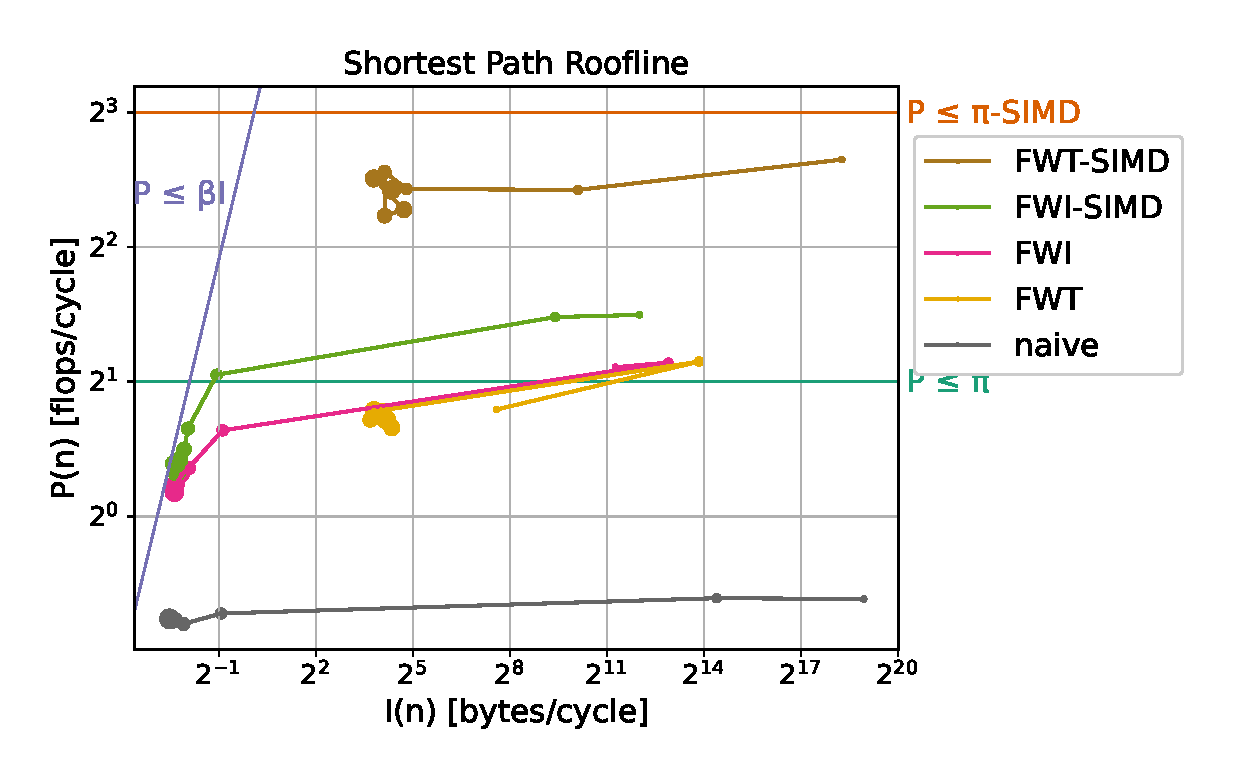
\includegraphics[width=0.47\textwidth, keepaspectratio=true]{sp-optimizations-large_roof.eps}
    \caption{Roofline plot of FW implementations for APSP.}
    \label{fig:sp-roof}
\end{figure}


\mypar{Max-Min Results}
As the structure of the computation, the instruction latency and throughput, as well as the data structure and representation
is identical to that of the APSP instance, we expect our optimizations to reach similar performance values for the MM instance.

Figure \ref{fig:mm-perf} shows the performance of the MM implementations. For scalar code, the tiled FWT code achieves
2.2x speedup relative to the naive implementation and 103\% of peak scalar performance because of the bug in the autotuner.
For vector code, the tiled FWT significantly outperforms the non-tiled counterpart and achieves 6.1x speedup relative to
the naive implementation and 72\% of the theoretical peak SIMD performance. 

Similarly to the APSP instance, the performance for both tiled implementations shows a dropoff at $N = 2304$. This is interesting
as it would be odd for the autotuner to manifest the same quirk to find a suboptimal local maximum for the same region of
input sizes. It is not impossible, however, as the performance for $N = 2880$ shows improvement which it did not do
for the APSP instance.

Looking at the roofline plot in figure \ref{fig:mm-roof} we find the same characteristic for the MM instance that only tiled
implementations manage to stay computationally bounded. This is an example of one autotuner being able to effectively
apply the same optimizations to two different algorithms.
\begin{figure}[h]
    \centering
    \includegraphics[width=0.47\textwidth, keepaspectratio=true]{mm-optimizations-large_perf.eps}
    \caption{Performance comparison of FW implementations for MM.}
    \label{fig:mm-perf}
\end{figure}
\begin{figure}[h]
    \centering
    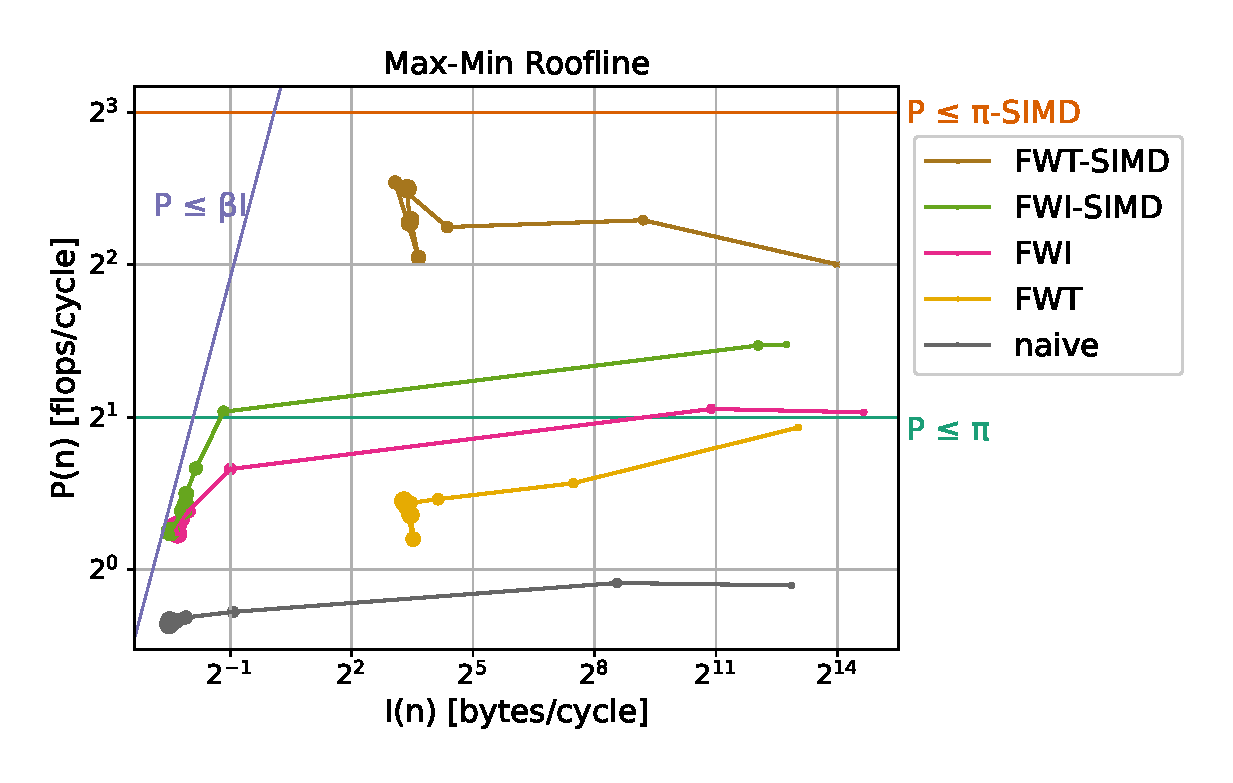
\includegraphics[width=0.47\textwidth, keepaspectratio=true]{mm-optimizations-large_roof.eps}
    \caption{Roofline plot comparing implementations for Max-Min on an Intel Core i7 (Coffee Lake microarchitecture).}
    \label{fig:mm-roof}
\end{figure}

\mypar{Transitive Closure Results}
The TC instance, while following the same algorithmic and data structure has a different data representation and instruction
latency and throughput. As a result, it is not a given that the optimizations translate to this instance.

Figure \ref{fig:tc-perf} shows the performance plot for the TC instance. The scalar FWT implementation achieves 65\% of the
theoretical scalar peak performance. However, due to finding and fixing a bug too close to the deadline, we were not able to run the measurements
for all input sizes as running the autotuner takes considerable amount of time, especially for the large input sizes. The
vectorized FWT implementation achieves a 33.3x speedup compared with the naive implementation and 65\% of the theoretical
SIMD peak performance.

Note that the vectorized tiled implementation exhibits large, intermittent dropoffs in performance. In this case we know that this
is caused by a constriction of the parameter space for certain input sizes leading to the optimal tiling factors not being available
for selection by the autotuner. The lack of legal optimal tiling factors is due to the bit-packing, which packs 256 bits into a
single vector register. Therefore, the number of available factors and therefore tiling factors diminishes considerably.

Looking at the roofline plot in figure \ref{fig:tc-roof} we see that, while both vectorized implementations initially display 
similar performance characteristics, the fact that,  like for the other instances, only the tiled implementations remain
compute-bound, the tiled implementation performs better for large input sizes.

This shows that the autotuner was still able to successfully apply the same optimizations and achieve a similar result
even for different data representations and different instruction latencies and throughputs. However, the TC instance
also shows limits to the generality of our autotuner. While the vectorized FWT remained compute bound, its performance
was severely decreased as a consequence of the different data representation with the bit-packed vectors.
However, the different instruction latencies and throughputs do not impact the performance, as an autotuner
finds the optimal values empirically.

\begin{figure}[h]
    \centering
    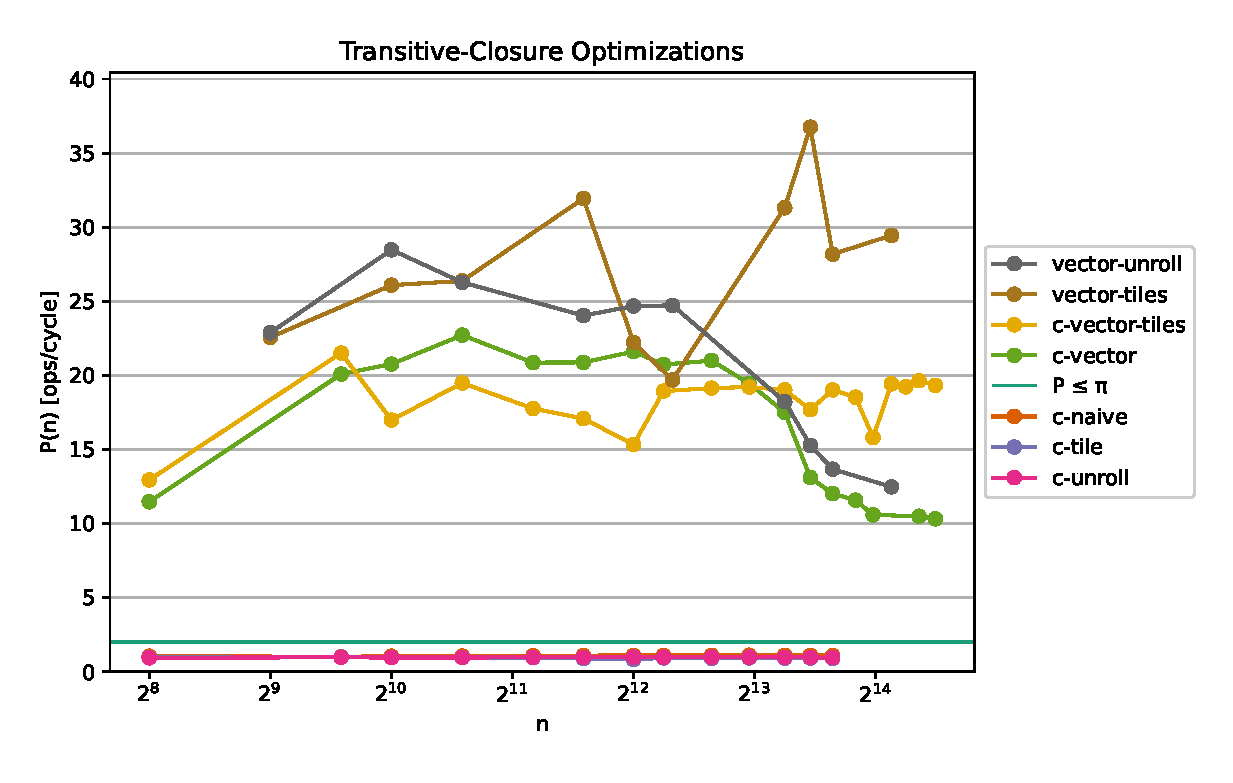
\includegraphics[width=0.47\textwidth, keepaspectratio=true]{tc-optimizations-large_perf.eps}
    \caption{Performance comparison of FW implementations for TC.}
    \label{fig:tc-perf}
\end{figure}
\begin{figure}[h]
    \centering
    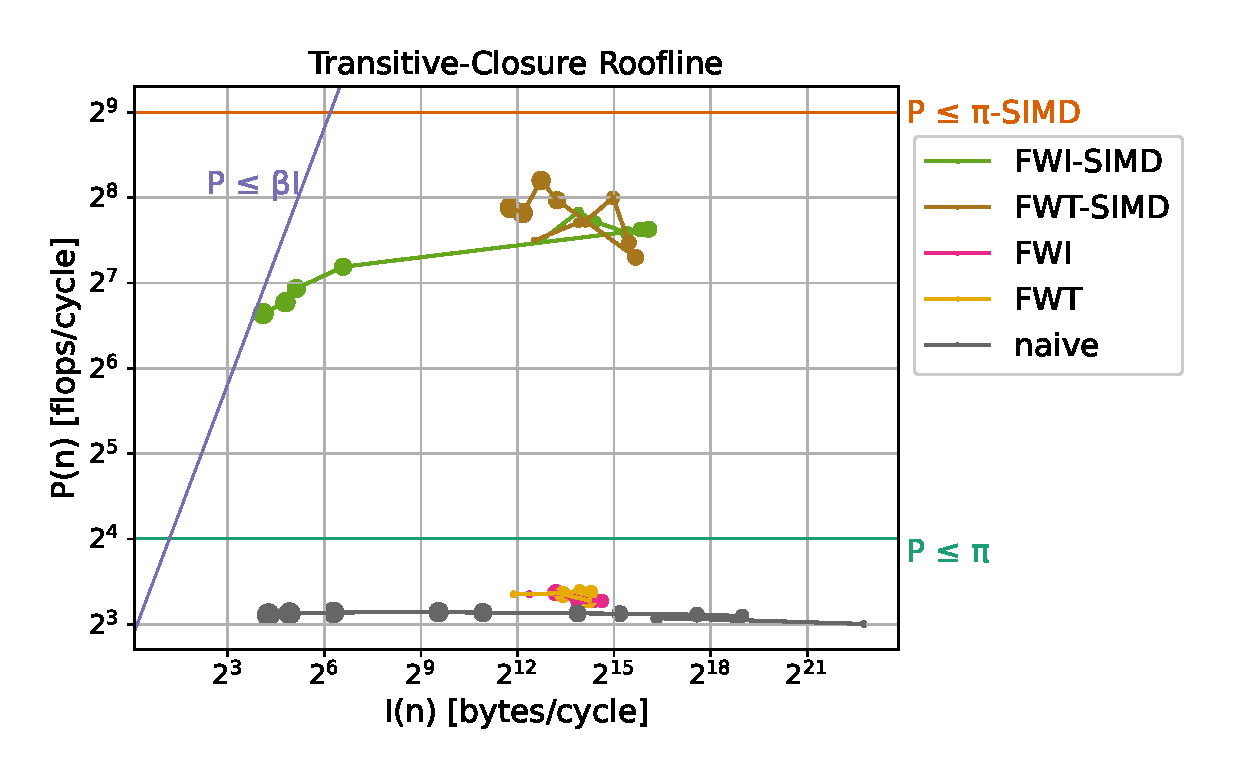
\includegraphics[width=0.47\textwidth, keepaspectratio=true]{tc-optimizations-large_roof.eps}
    \caption{Roofline plot comparing implementations for Transitive Closure on an Intel Core i7 (Coffee Lake microarchitecture).}
    \label{fig:tc-roof}
\end{figure}
\section{Conclusions}
To summarize, we examined three instances of the generalized Floyd-Warshall algorithm. Respectively, they solve the all-pairs shortest-path, widest-path and transitive closure problems. We implemented various optimizations for each, namely \texttt{FWI}, \texttt{FWT}, and corresponding vectorized versions.
Finally, we implemented an autotuner that finds locally optimal unrolling and tiling factors and generates corresponding code.

Our benchmarks confirm that the optimization techniques for the all-pairs shortest-path problem by Han, Franchetti and Püschel \cite{han06generation} work, and we show that they generalize to the other two examined closed semi-rings of the widest-path and transitive closure instances. Further, we showed that a single autotuner implementation is
able to successfully apply the same optimizations to all three problems.

However, we also found limits to the generality of our autotuner as soon as the data representation changes.
This leads us to conjecture that our autotuner should be easily generalizable to other closed semi-rings over
$\mathbb{R}^\infty$.

\mypar{Future Work}
An obvious next step would be to implement other closed semi-rings in our autotuner. A good choice would be
the unpivoted Gauss-Jordan transform, as it is a semi-ring over $\mathbb{R}\cup\{\text{undefined}\}$. For further
generalization we would likely need an autotuner which is aware of the program structure and is able to apply
transforms based on the structure as needed for different data representations. Ideally, one would implement
an autotuner fully generic over a closed semi-ring.

There are also more optimizations that could be applied to the Floyd-Warshall algorithm. One example is the
doubly tiled version described by Han et al. \cite{han06generation}. Another possible optimization would be
to explore different algorithms for matrix closure. One possible candidate might be R-Kleene 
\cite{dalberto2007r-kleene}.

%\section{Further comments}

{\color{red}TODO: Remove}
Here we provide some further tips.

\mypar{Further general guidelines}

\begin{itemize}
\item For short papers, to save space, I use paragraph titles instead of
subsections, as shown in the introduction.

\item It is generally a good idea to break sections into such smaller
units for readability and since it helps you to (visually) structure the story.

\item The above section titles should be adapted to more precisely
reflect what you do.

\item Each section should be started with a very
short summary of what the reader can expect in this section. Nothing
more awkward as when the story starts and one does not know what the
direction is or the goal.

\item Do not use subsubsections.

\item Make sure you define every acronym you use, no matter how
convinced you are the reader knows it.

\item Always spell-check before you submit.

\item Be picky. When writing a paper you should always strive for 
high quality. Many people may read it and the quality makes a big difference.
In this class, the quality contributes to the grade.

\item Books helping you to write better: \cite{Higham:98} and \cite{Strunk:00}.
\end{itemize}

\mypar{Graphics} For plots that are not images {\em never} generate (even as intermediate step)
jpeg, gif, bmp, tif. Use eps, which means encapsulate postscript, or pdf. This way it is
scalable since it is a vector graphic description of your graph. E.g.,
from Matlab, you can export to eps or pdf.

Fig.~\ref{fftperf} is an example plot that I used in a lecture. Note that the fontsize in the plot should not be any smaller. On the other hand it is also a good rule that the font size in the plot is not larger than the one in the caption (otherwise it looks ugly).

\begin{figure}\centering
  \includegraphics[scale=0.33]{dft-performance.pdf}
  \caption{Performance of four single-precision implementations of the
  discrete Fourier transform. The operations count is roughly the
  same. {\em The labels in this plot are about the smallest you should go.}\label{fftperf}}
\end{figure}

\bigskip
{\bf Up to here you have 8 pages.}

\section{Contributions of Team Members}

In this section we briefly list what each team member contributed to the project in terms of code written for optimization and analysis. Please note that while infrastructure- and testing-related code is not included here, props go out to Manuel for setting up an awesome build system utilizing Docker containers to ensure identical dependencies and to Florian for setting up a highly-convenient, all-powerful development pipeline.

\mypar{Florian} I built the foundation of the autotuner including generic code templates for all three algorithms with cache tiling, loop unrolling and vectorization. The autotuner is initially using an exhaustive search and then applies hill climbing to find the optimal parameters.

\mypar{Roman}
I added bit-packing to the transitive closure infrastructure by adjusting the code to read and write input, and the naive implementation. I wrote the initial vectorized versions for all three problems. I helped in applying other optimizations to transitive closure, and fixing some of the problems that arose in the process.

\mypar{Manuel} I set up the measurements using PAPI counters needed for the plots and the autotuner. I polished Florian's initial autotuner implementation with an improved hill climbing algorithm. Further, I applied and fine-tuned optimizations for the shortest path implementation.

\mypar{Lasse} I implemented vectorized and non-vectorized versions of the FW, FWI, FWIabc and FWT algorithms for the widest-path, that is, Max-Min, algorithm. I supported Manuel and Roman in applying FWI and FWT optimizations to their programs and built on Manuel's and Florian's work to integrate FWT optimizations and vectorization in the final version of the autotuner.

%{\color{red}TODO: REMOVE}
%In this mandatory section (which is not included in the 8 pages limit) each team member should very briefly (telegram style is welcome) explain what she/he did for the project. I imagine this section to be between one column and one page (absolute maximum).
%
%Include only 
%\begin{itemize}
%	\item What relates to optimizing your chosen algorithm / application. This means writing actual code for optimization or for analysis.
%	\item What you did before the submission of the presentation.
%\end{itemize}
%Do not include
%\begin{itemize}
%	\item Work on infrastructure and testing.
%	\item Work done after the presentation took place.
%\end{itemize}
%
%Example and structure follows.
%
%\mypar{Marylin} Focused on non-SIMD optimization for the variant 2 of the algorithm. Cache optimization, basic block optimizations, small generator for the innermost kernel (Section 3.2). Roofline plot. Worked with Cary and Jane on the SIMD optimization of variant 1, in particular implemented the bit-masking trick discussed.
%
%\mypar{Cary} ...
%
%\mypar{Gregory} ...
%
%\mypar{Jane} ...

% References should be produced using the bibtex program from suitable
% BiBTeX files (here: bibl_conf). The IEEEbib.bst bibliography
% style file from IEEE produces unsorted bibliography list.
% -------------------------------------------------------------------------
\bibliographystyle{IEEEbib}
\bibliography{bibl_conf}

\newpage

\appendix

\section{Appendix}

\subsection{Code Samples}\label{app:code}
\begin{listing}[h!]
\caption{An unrolled implementation of the APSP FW instance.}\label{lst:unrolled}
\begin{minted}{c}
int floydWarshall(double *C, int N) {
  for (int k = 0; k < N; k++) {
    for (int i = 0; i < N; i ++) {
      double cik = C[i * N + k];
      for (int j = 0; j < N - 1; j += 2) {
        // load
        double cij0 = C[i * N + j + 0];
        double cij1 = C[i * N + j + 1];

        double ckj0 = C[k * N + j + 0];
        double ckj1 = C[k * N + j + 1];

        // compute 1
        double sum0 = cik + ckj0;
        double sum1 = cik + ckj1;

        // compute 2
        double res0 = MIN(cij0, sum0);
        double res1 = MIN(cij1, sum1);

        // store
        C[i * N + j + 0] = res0;
        C[i * N + j + 1] = res1;
      }
    }
  }
  return 0;
}
\end{minted}
\end{listing}

\subsection{Autotuner Parameter Choices}
The following are the autotuner's choices of unrolling factors and tile sizes, all stemming from the MM instance.
In the tables, N denotes the input size, $L_1$ the tile size, and $U_{i, j, k}$ the unrolling factors of the various loops.

In the case of \texttt{FWT}, the unrolling factors $U_{i, j}$ concern the function \texttt{FWI}, and the unrolling factors $U_{i, j, k}'$ concern the function \texttt{FWIabc}.

\begin{table}[h]
\centering
\begin{tabular}{|c|c|c|}
\hline
N & $U_i$ & $U_j$ \\
\hline
432 & 3 & 1\\
576 & 3 & 1\\
1152 & 3 & 1\\
1728 & 3 & 1\\
2304 & 3 & 1\\
2880 & 3 & 1\\
3456 & 3 & 1\\
4032 & 3 & 1\\
\hline
\end{tabular}
\caption{Parameters for scalar \texttt{FWI}}
\end{table}

\begin{table}[h]
\centering
\begin{tabular}{|c|c|c|c|c|c|c|}
\hline
N & $L_1$ & $U_i$ & $U_j$ & $U_i'$ & $U_j'$ & $U_k'$ \\
\hline
432 & 144 & 3 & 1 & 1 & 9 & 16\\
576 & 576 & 3 & 1 & 1 & 8 & 18\\
1152 & 96 & 3 & 1 & 1 & 8 & 16\\
1728 & 144 & 3 & 1 & 1 & 8 & 18\\
2304 & 96 & 1 & 1 & 1 & 8 & 16\\
2880 & 192 & 2 & 1 & 1 & 6 & 4\\
3456 & 128 & 2 & 1 & 1 & 8 & 16\\
4032 & 224 & 2 & 1 & 1 & 8 & 16\\
\hline
\end{tabular}
\caption{Parameters for scalar \texttt{FWT}}
\end{table}

\begin{table}[h]
\centering
\begin{tabular}{|c|c|c|}
\hline
N & $U_i$ & $U_j$ \\
\hline
432 & 4 & 8\\
576 & 3 & 4\\
1152 & 8 & 4\\
1728 & 9 & 4\\
2304 & 8 & 4\\
2880 & 8 & 4\\
3456 & 4 & 12\\
\hline
\end{tabular}
\caption{Parameters for vectorized \texttt{FWI}}
\end{table}

\begin{table}[h]
\centering
\begin{tabular}{|c|c|c|c|c|c|c|}
\hline
N & $L_1$ & $U_i$ & $U_j$ & $U_i'$ & $U_j'$ & $U_k'$ \\
\hline
432 & 144 & 9 & 4 & 4 & 12 & 16\\
576 & 96 & 8 & 8 & 4 & 16 & 16\\
1152 & 96 & 8 & 4 & 4 & 8 & 16\\
1728 & 144 & 8 & 4 & 4 & 8 & 16\\
2304 & 96 & 4 & 4 & 3 & 16 & 16\\
2880 & 192 & 8 & 8 & 4 & 8 & 16\\
3456 & 128 & 8 & 4 & 4 & 16 & 16\\
4032 & 192 & 8 & 4 & 4 & 8 & 16\\
\hline
\end{tabular}
\caption{Parameters for vectorized \texttt{FWT}}
\end{table}

\end{document}
